%!TEX root = ../thesis.tex


\begin{figure}[!b]
    \centering
    \begin{subfigure}[b]{0.8 \textwidth}
        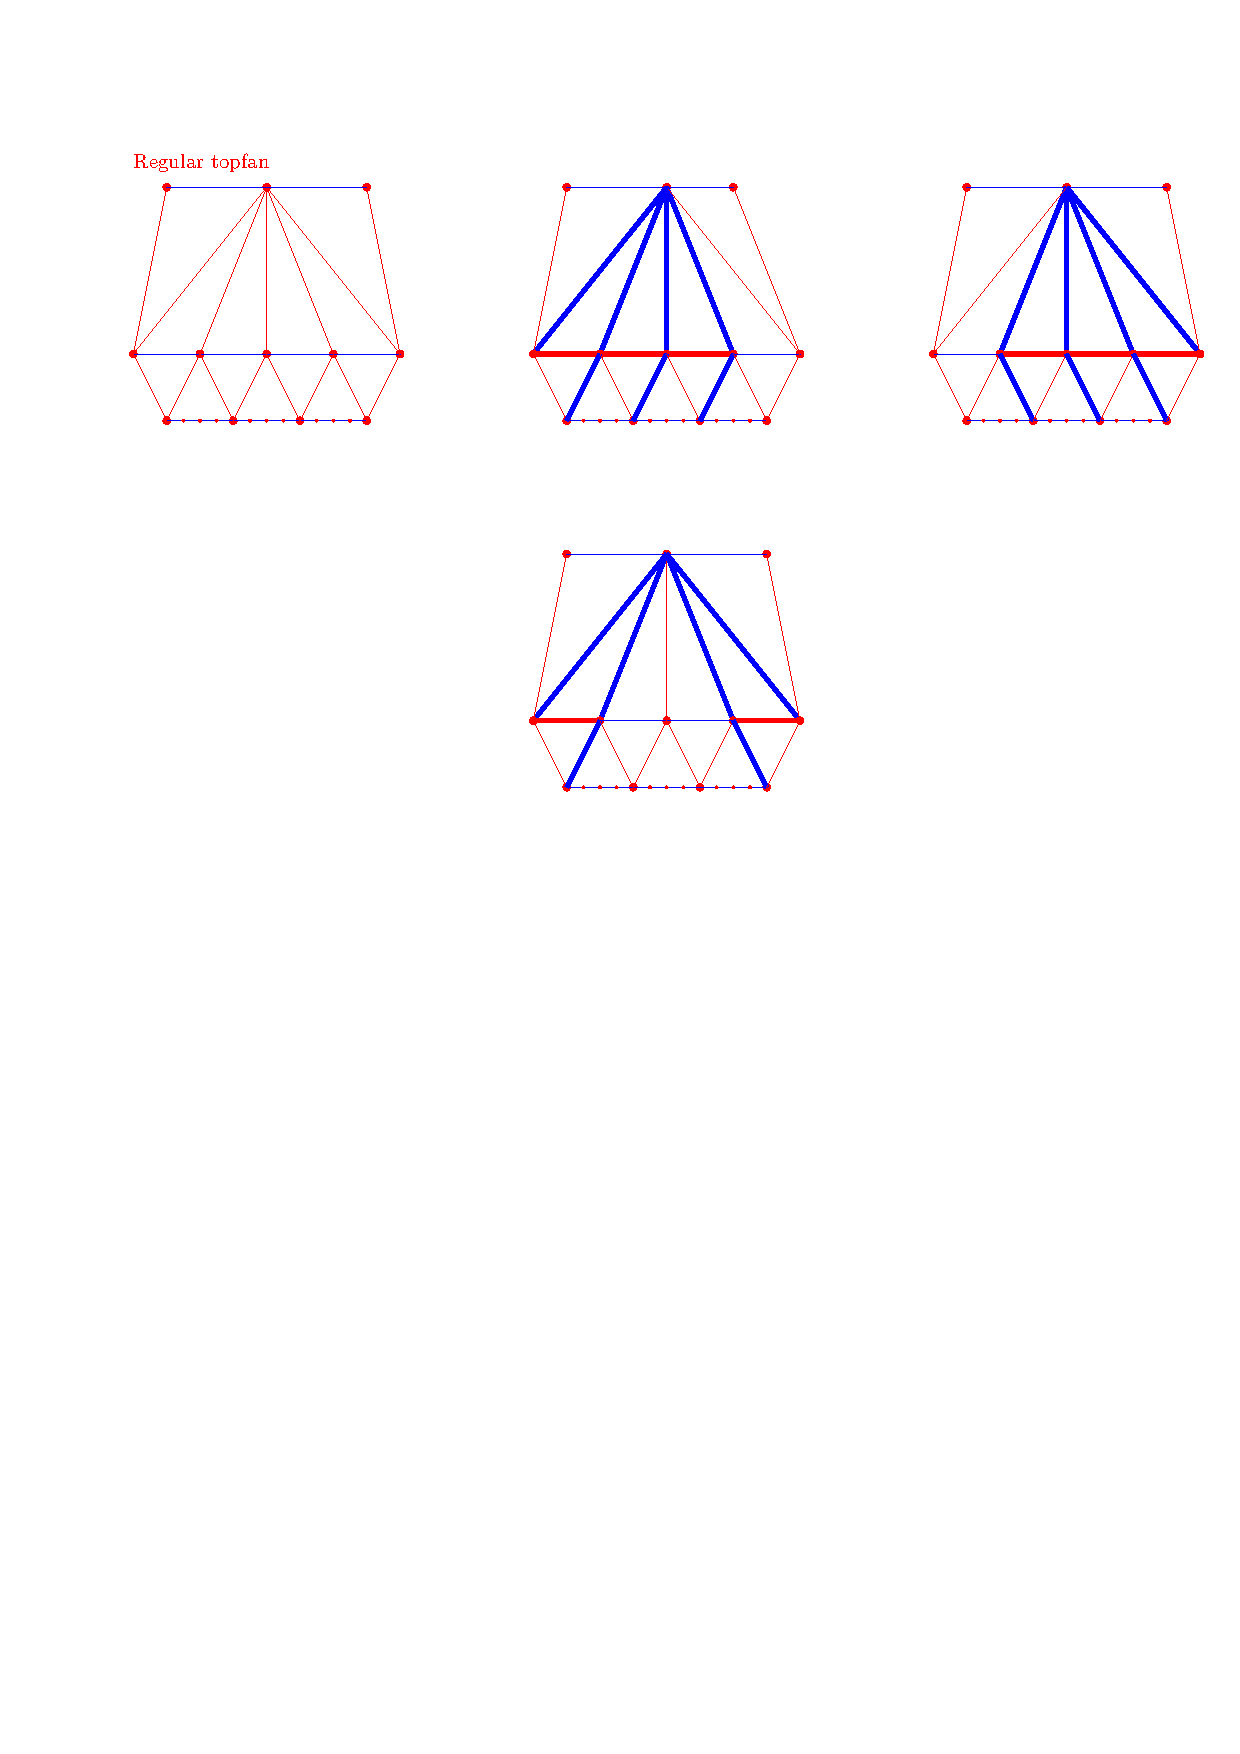
\includegraphics[width = \textwidth]{topFanFlips/img/regular}
        \caption{The regular topfanflip.}
        \label{fig:fanflip:regular}
    \end{subfigure}
    ~
    \centering
    \begin{subfigure}[b]{0.45 \textwidth}
        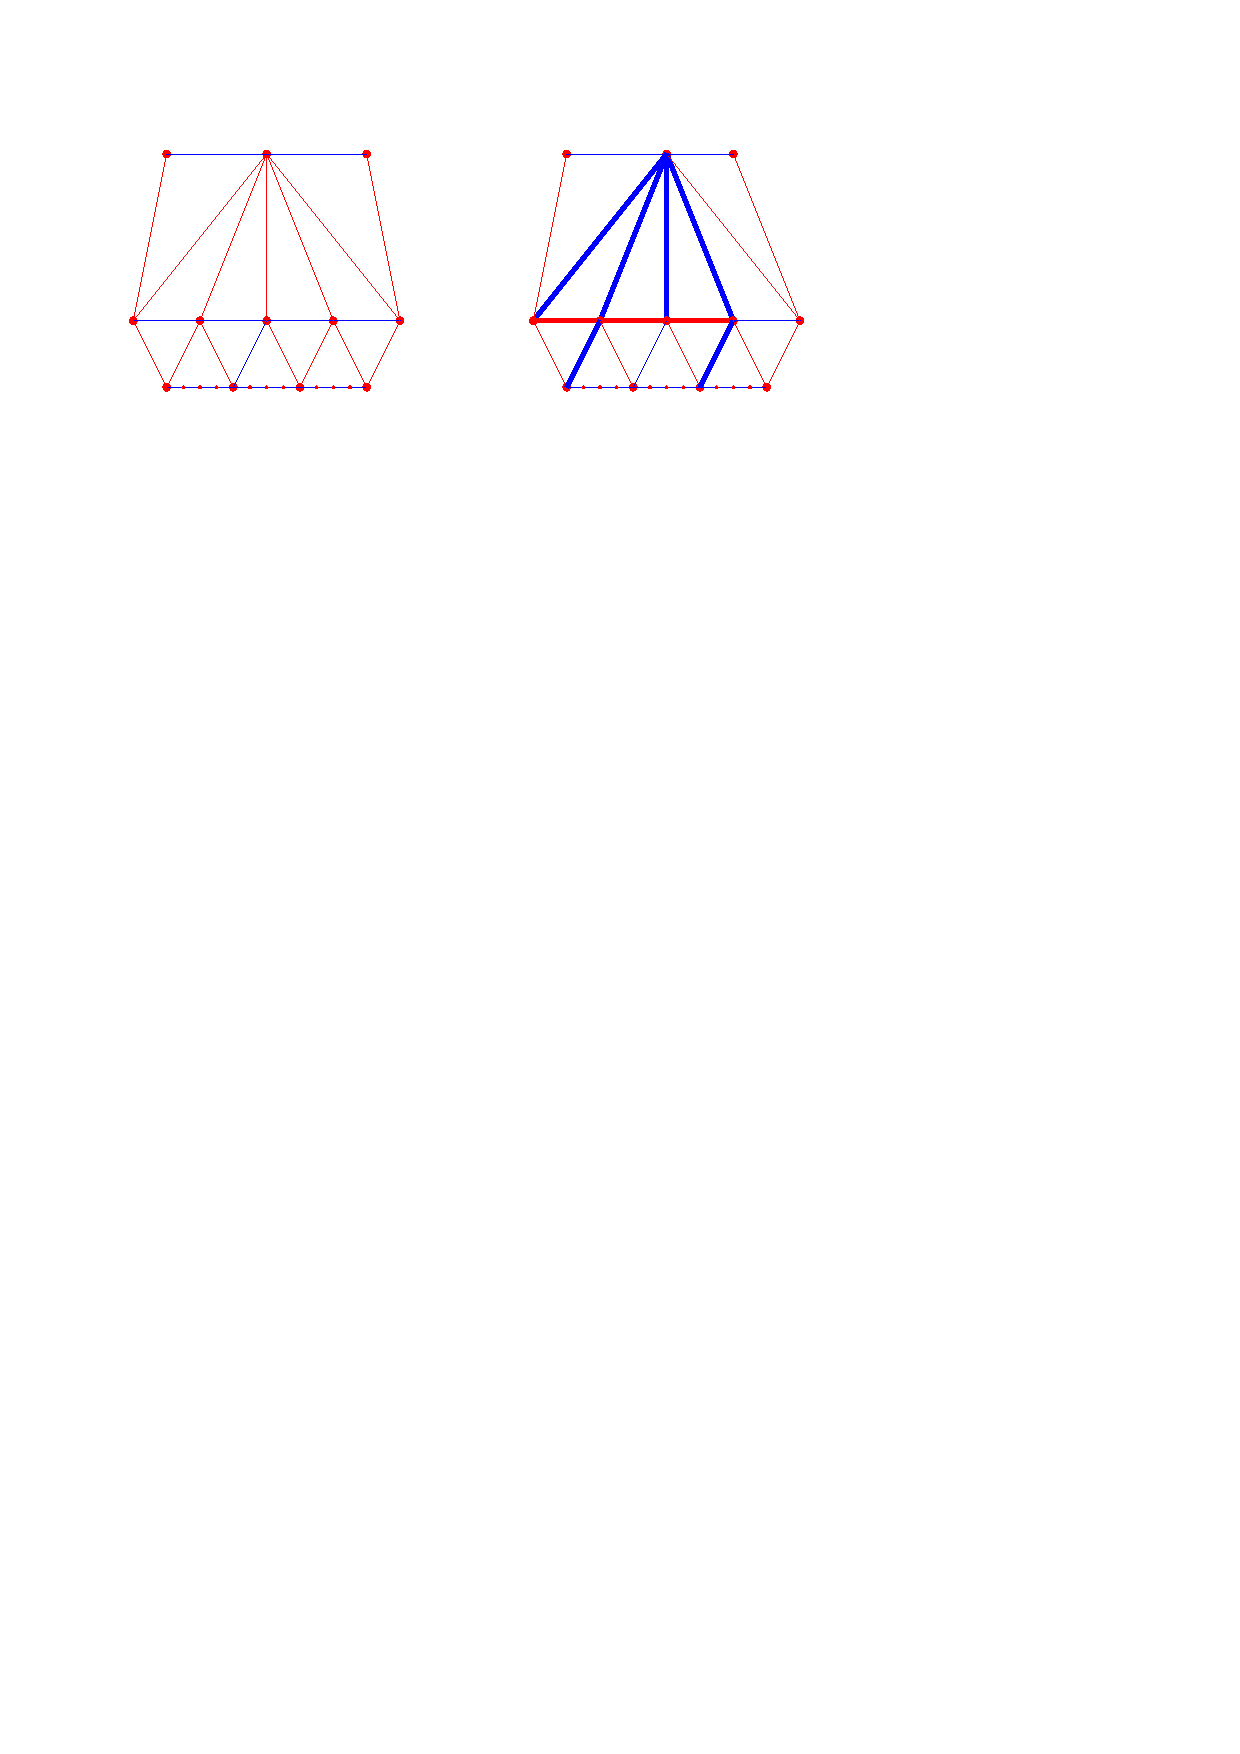
\includegraphics[width = \textwidth]{topFanFlips/img/merge}
        \caption{Topfanflip above a merge.}
        \label{fig:fanflip:merge}
    \end{subfigure}
    ~
    \begin{subfigure}[b]{0.45 \textwidth}
        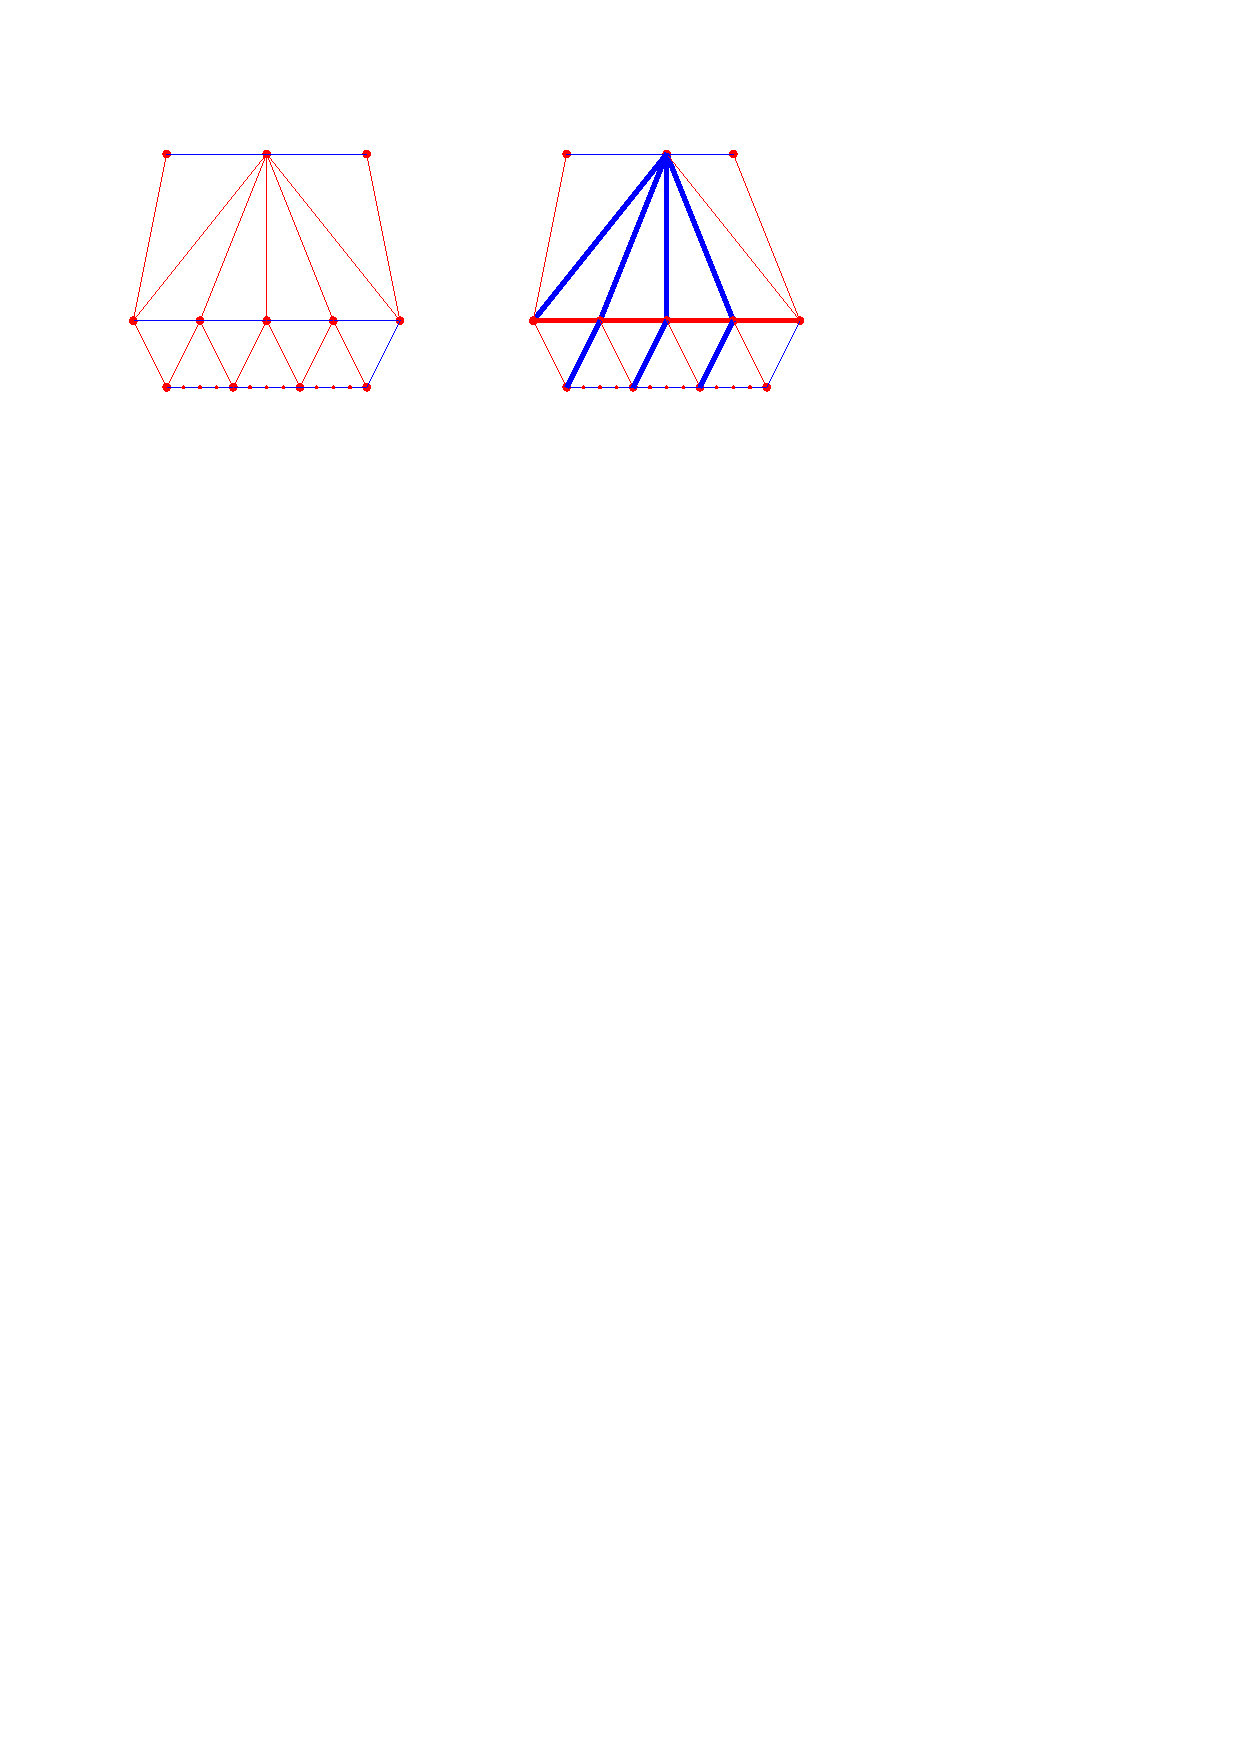
\includegraphics[width =\textwidth]{topFanFlips/img/mergeend}
        \caption{Topfanflip next to merge. Note the additional red edge.}
        \label{fig:fanflip:mergeLastVertex}
    \end{subfigure}
    \centering
    \begin{subfigure}[b]{0.45 \textwidth}
        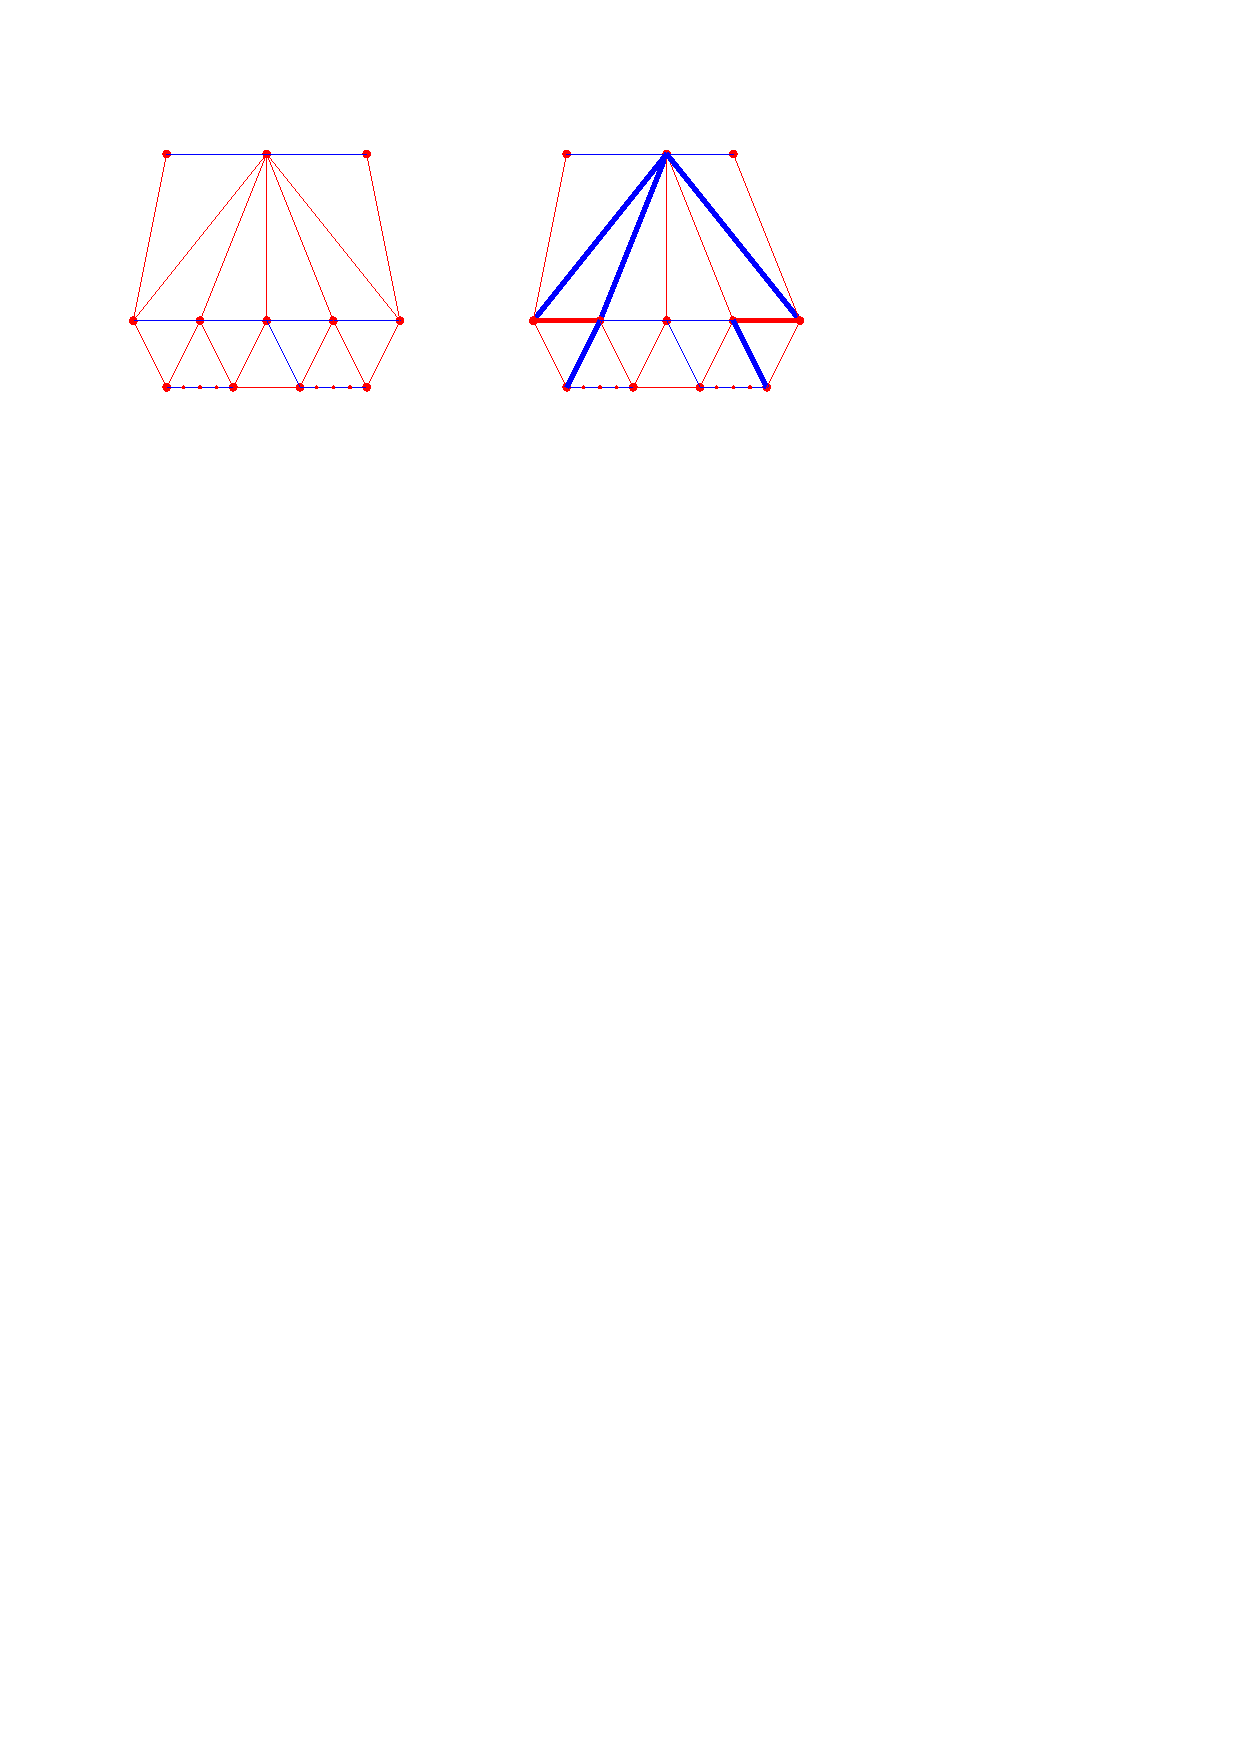
\includegraphics[width = \textwidth]{topFanFlips/img/split}
        \caption{Before a split we stop.}
        \label{fig:fanflip:split}
    \end{subfigure}
    ~
    \begin{subfigure}[b]{0.45 \textwidth}
        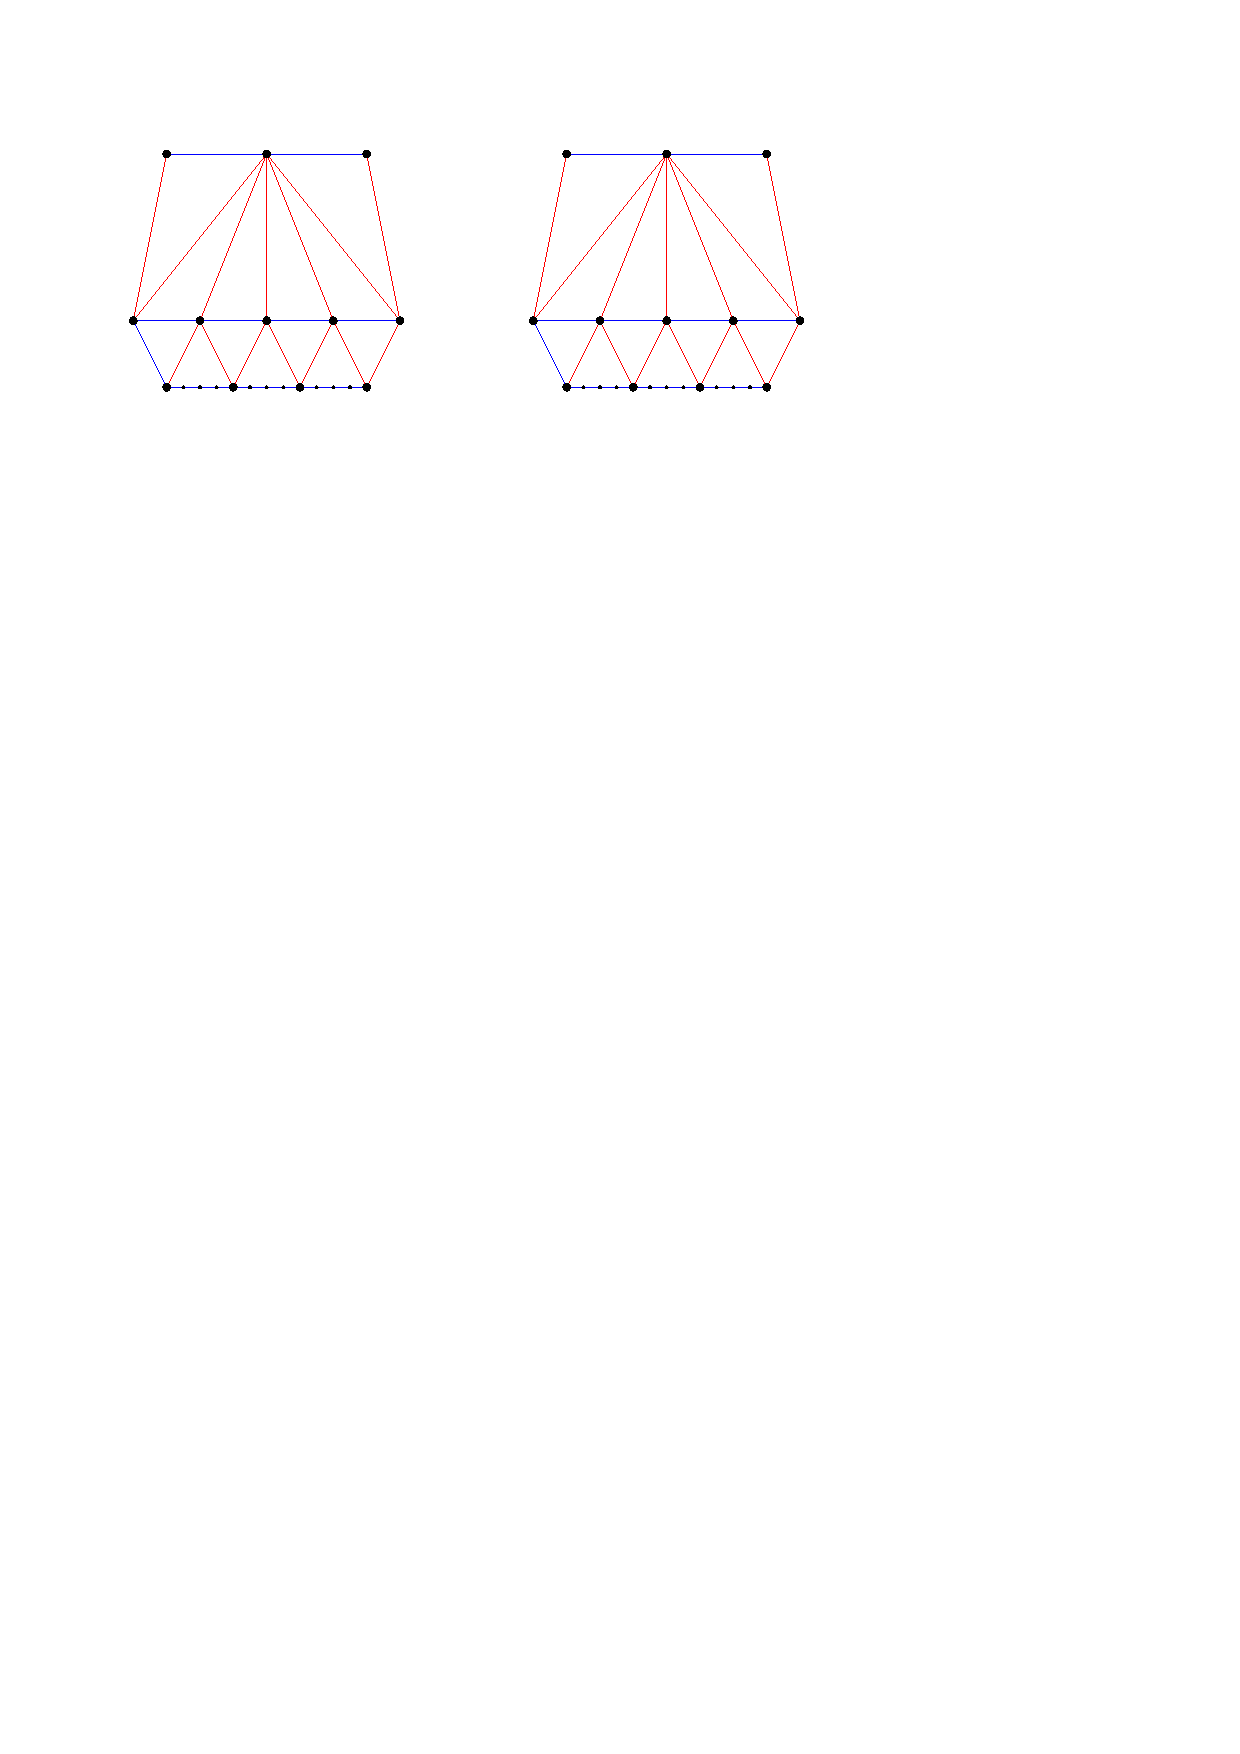
\includegraphics[width =\textwidth]{topFanFlips/img/splitfront}
        \caption{If the split is on the first vertex we do not flip at all.}
        \label{fig:fanflip:splitFirstVertex}
    \end{subfigure}

    \caption{Topfan Flips.}
    \label{fig:fanflip:fanflips}
\end{figure}

\subsection{Topfan flips}
\thispagestyle{plain}
\label{ss:fanflip}

In Section \ref{ss:flipBlueZ} we obtained a vertically one-sided regular edge labeling (Lemma \ref{lm:sweep:vertOnsided}).
Moreover, this regular edge labeling never has a split next to a topfan handle along the rightmost edge of the split (Lemma \ref{lm:zflip:NoTwoSplitsAboveEachOtherVertOnesided}).

Using local recoloring (\emph{flips}) on the topfans we will maintain a one-sided regular edge labeling (Lemma \ref{lm:topfan:oneSidedREL}) and make sure that large topfans only occur in very specific situations (Lemma \ref{lm:topfan:remainingTopfans}). It will turn out that we can deal with these specific situations in the final step of Section \ref{ss:subdiv}.

Our flips differ depending on whether we we encounter a split and or merge in the bottom boundary path. Refer to Figure \ref{fig:fanflip:fanflips} for a first glance at the different kinds of topfanflips.





%\fxnote{We could make structure of the fence below the topfan more explicit. But we do not really need this}

\mypar{In what order to flip topfans}
We consider all faces we have in order from last created to first created. Since a topfan flip only affects the current face and faces below it we never have to flip in a faces that is affected by the results of a topfan flip.
We do not flip topfans whose fanhandle is adjacent to the merge of the face.

\mypar{How to flip a topfan}
A topfan is above a number of edges of the bottom fence of the face containing the topfan. These edges are the rim of the fan. We will call a vertex \emph{$\pS$-adjacent} if it adjacent to $\pS$.

We flip the topfan along the rim starting at the first vertex and ending at the the vertex \textbf{before} the first splitvertex or $\pS$-adjacent vertex or the vertex \textbf{before} the last vertex. This can imply that we do not flip any edges (in the case that the first vertex is a split vertex or $\pS$-adjecent).

We will use the notation introduced in figure \ref{fig:fanflip:regular}.
For the first vertex $v_1$ we recolor the adjacent outer edge of the topfan. For subsequent vertices $v_i$ we recolor the rim edge between this vertex and the previous vertex $v_{i-1}$ red and we recolor the both edges directly adjacent to this edge in the rotation at $v_i$ blue (if they weren't already blue).
If we stop flipping before a merge vertex $v_{i+1}$ we flip an additional edge $v_i v_{i+1}$ along the rim.


\mypar{Examples}
Let us show a few example of this procedure to improve clarity.
If the rim has no merges or splits we execute the topfanflip depicted in Figure \ref{fig:fanflip:regular}. We color all but the rightmost fan edge blue, color all but the rightmost rim edge red. And color the left sides of all topfans below this topfan in the face below the current face blue.

If the rim consists of only merges we easily adept a topfanflip to this situation. We simply do not flip the edge merging in as depicted in Figure \ref{fig:fanflip:merge}.

A special case is given by a merge on the last vertex on the bottom edges of the topfan. In that case we flip all rim edges (even the last one) to prevent a blue $Z$ from forming. See figure \ref{fig:fanflip:mergeLastVertex}.

Splits are more difficult to handle. We are unfortunately unable to keep flipping once we hit a split hence we stop before we get that far. See Figure \ref{fig:fanflip:split}. It this happens on the first vertex we do not flip at all, see Figure \ref{fig:fanflip:splitFirstVertex}.

\mypar{The result}
Before the topfanflips we had a vertically one-sided regular edge labeling. Afterwards we still have a vertically one-sided regular edge labeling, as we will prove in Lemma \ref{lm:topfan:oneSidedREL}. Moreover we have no large top-fans except for some controlled cases (Lemma \ref{lm:topfan:remainingTopfans}).

\begin{lemma}
  \label{lm:topfan:oneSidedREL}
  The regular edge labeling is still vertically one-sided after a topfanflip
\end{lemma}
\begin{proof}
  We take another look at Figure \ref{fig:fanflip:fanflips}. Note that due to Lemma \ref{lm:zflip:blueZNorVertOneSided} that we are vertically one-sided as long as there is no blue $Z$.  Since the graph was one-sided we can assume that we had no blue $Z$'s.
  Let us first consider the regular case. Since the edge  $v_n w_m$ is red (otherwise we would have a merge) this change does not produce any blue $Z$'s.

  Let us also consider the merge cases. Due to the clever recoloring these also do not lead to a blue $Z$.
  %However they can lead to a face starting with a large topfan. We will later see this is a controlled topfan.
  It is clear the split cases also do not produce a blue $Z$.
  Since any south-adjecnt fan is treated like a split fan we also do not create $Z$'s in these cases.
  %But the topfans are again controlled. As we will see in the next section.
\end{proof}


\begin{lemma}
  \label{lm:topfan:remainingTopfans}
  In the remaining faces every large topfan is in one of the following two situations.
  \begin{enumerate}
    \item  This topfan is at the start of the face
    \item  The left outer rim vertex is a splitvertex.
  \end{enumerate}
\end{lemma}
\begin{proof}
  All topfans are manipulated in such a way that they start a new face, or are colored blue entirely, unless the left outer rim vertex is a split. Since in that case we do not flip at all, but then the left outer rim vertex is indeed a split.
\end{proof}
